\documentclass[14pt]{article}
\usepackage[margin=1in]{geometry}
\usepackage{amsmath}
\usepackage{amssymb}
\usepackage{fancyhdr}
\usepackage{graphicx}
\usepackage{xcolor}
\usepackage{hyperref}
\usepackage{tikz}
\renewcommand{\familydefault}{\sfdefault}
\parindent 0ex
\everymath{\displaystyle{}}

\title{ENGG 202\\Engineering Statics}
\author{Andy Smit}
\date{Winter 2019}

\begin{document}
    \maketitle
    \section{Equilibrium Equation:}
    $\sum F_x=0$ $\sum F_y=0$ $\sum M=0$
    \subsection{Free Body Diagram}
    Diagram representation of the isolated system treated as a single
    body. We model forces exerted on the body to be isolated by the body
    removed. If a support prevents translation (or rotation) in a given
    direction     
    \section{Statical Determinacy}
    \textbf{Constraint: } Restriction of movement\\
    \textbf{Statically Determinant System: }All unknown external effects
    can be determined from equilibrium conditions.\\
    \textbf{Degree of Statical Indeterminacy: }The number of redundant
    reaction forces is equal to the number of all constraints minus the
    number of equilibrium conditions.\\
    \textbf{Two and Three Force Members}: A body is in equilibrium under
    the action of two (three) forces only. A force member must have
    equal, opposite and colinear forces.\\
    \textbf{Three Force Member}:\\
    
    \begin{figure}[h]
        \caption{A 3 force Member}
        \begin{tikzpicture}
            \draw (0,0) circle [x radius=2, y radius=1];
            \draw[color=red] [<-] (0,1)--(0, 2); \draw[color=red] [<-]
            (315:1)--(315:2); \draw[color=red] [<-] (225:1)--(225:2);
        \end{tikzpicture}
    \end{figure}
    \begin{figure}[h]
        \caption{A 2 Force Member}
        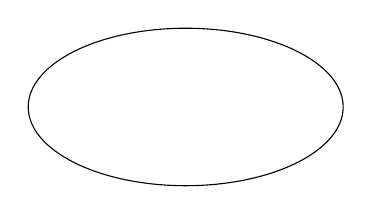
\begin{tikzpicture}
            \draw (0,0) circle [x radius=2, y radius=1];
        \end{tikzpicture}

    \end{figure}
    \section{3D Vectors}
    \textbf{Dot Product:}\\
    If $\vec{A}$ and $\vec{B}$ are two vectors where
    $\vec{A}=\begin{pmatrix}A_1\\A_2\\A_3 \end{pmatrix}$ and
    $\vec{B}=\begin{pmatrix}B_1\\B_2\\B_3\end{pmatrix}$ then the dot
    product between $\vec{A}$ and $\vec{B}$ is defined:
    $$\vec{A}\cdot
    \vec{B}=A_1B_1+A_2B_2+A_3B_3=||\vec{A}||\,||\vec{B}||\cos\theta$$
    \textbf{Cross Product:}\\
    If $\vec{A}=\begin{pmatrix}A_1\\A_2\\A_3 \end{pmatrix}$ and
    $\vec{B}=\begin{pmatrix}B_1\\B_2\\B_3\end{pmatrix}$ are two vectors
    in $\mathbb{R}^3$ then the cross product $\vec{A}\times\vec{B}$ is
    defined either geometrically as
    $$||\vec{A}\times\vec{B}||=||\vec{A}||\,||\vec{B}||\sin\theta$$ or
    algebraically as $$\vec{A}\times\vec{B}=\begin{vmatrix} \hat{i} &
    \hat{j} &\hat{k}\\
        A_1 & A_2 & A_3\\
        B_1 & B_2 & B_3 \end{vmatrix}$$ \textbf{Projections:}\\
    $F_n=F\cos\theta=\vec{F}\cdot\vec{n}$\\
    \textbf{Moment In 3D: }\\
    $\vec{M_O}=\vec{r}\times\vec{F}$\\\\
    \textbf{Moment about an Arbitrary axis:}\\
    Let $\lambda$ be some arbitrary axis passing through point $O$ then
    the moment about point $O$ about $\lambda$ is 
    $$M_\lambda=(\vec{r}\times\vec{F})\cdot\vec{n}$$ where $\vec{n}$ is
    a unit vector in the direction of $\lambda$, $\vec{r}$ is the
    position vector between the application of the Force and $O$, and
    $\vec{F}$ is the force applied. In 2 and 3D the moment produced by a
    force going through a point $A$ about point $A$ is $0$. In 3D if a
    force is parallel or concurrent with the axis $\lambda$ then the
    moment about $\lambda$ is $0$.\\\\
    \textbf{Couple's In 3D:}\\
    $M_O=\vec{r_A}\times\vec{F}=\vec{r_B}\times\vec{F}=\vec{r}\times\vec{F}$\\
    \textbf{Force Couple System in 3D:}\\
    \textbf{Resultants in 3D:}\\
    General case (Non-concurrent Forces): 
    
    System of concurrent Forces:
    $$\sum\vec{F}=\vec{R}$$$$\vec{M_O}=0$$ System of Coplanar Forces:
    Same as 2D problem
    \section{Trusses}
    A truss is a group of members in tension and compression. Consists
    of many zero force members.
    \subsection{Method of sections:}
    Cut through members of a structure and consider its section.
    Determine all external reactions acting on the the truss system
    (This step may or may not be necessary). Make a cut creating two
    sections of 3 members max. Choose either side of the truss after
    cutting to solve for the forces acting on it.

    \section{Centroids and Center of Gravity}
    \subsection{Centroids:} The geometric center of a body
    \subsection{Center of Mass (CoM):} A point about which the every
    particle of its mass is equally distributed (center of a sphere).
    The  of all mass of an object. \subsection{Center of Gravity (CoG):}
    A point in the body where the whole weight of the body is acting.
    $$W=m g$$ Generally the center of mass is the same as the center of
    gravity for a uniform gravitational field. In all circumstances
    dealt with in this course center of mass is the same as center of
    gravity. In a homogeneous (uniform density) body the center of mass
    and the centroid are located at the same point. 
    \subsection{Determining the center of gravity}
    \subsubsection{Experimental Determination:}
    Hanging Mass Experiment: Hang a mass on a string in multiple
    orientations. When it reaches equilibrium the tension in the cable
    will be colinear with the weight of the object. After doing this at
    3 points the center of mass can be determined.
    \subsubsection{Mathematical Derivation:}
    Consider a body as a infinite number of particles with differential
    weight $dW$. The resultant weight is equal to the sum of all the
    infinitesimal weights. $$W=\int dW$$ In this case we can create a
    couple system between the origin and each particle. This couple has
    a force $W=\int dW$ and a moment $$\sum M_x=-\int y_c\, dW$$ From
    this we can determin that $$M_x=-\bar {y_c}W$$ where $\bar{y_c}$ is
    the distance from the axis to the center of gravity. Then
    understanding that the sum of moments is the same as the moment of
    sum, the following result can be obtained $$\bar y=\frac{\int y_c\,
    dW}{W}$$. For all coordinets the center of gravity is $$\bar
    x=\frac{\int x_c\, dW}{W}\ \  \bar y=\frac{\int y_c\, dW}{W}\ \ \bar
    z=\frac{\int z_c\, dW}{W}$$
    \subsection{Center of Mass Location:}
    The center of mass is determined using the same formula as center of
    gravity
    $$\bar x=\frac{\int x_c\, dW}{W}\ \  \bar y=\frac{\int y_c\, dW}{W}\
    \ \bar z=\frac{\int z_c\, dW}{W}$$ Now as express $W=mg$ and
    $dW=g\cdot dm$, then the formula becomes
    $$\bar x=\frac{\int x_c\, dm}{m}\ \  \bar y=\frac{\int y_c\, dm}{m}\
    \ \bar z=\frac{\int z_c\, dm}{m}$$ Finally recall that $m=\rho V$
    and $dm=\rho dV$
    $$\bar x=\frac{\int x_c\, \rho dV}{\int \rho dV}\ \  \bar
    y=\frac{\int y_c\, \rho dV}{\int \rho dV}\ \ \bar z=\frac{\int z_c\,
    \rho dV}{\int \rho dV}$$ The vector form the the location of the
    center of mass is given by $$\begin{pmatrix} \bar x\\ \bar y\\ \bar
    z \end{pmatrix}$$ When computing center of gravity choose the
    easiest coordinate system to use and planes of symmetry. If it makes
    things easier convert the coordinate system to a polar coordinate
    system 
    $$\left\{\begin{array}{lr} x=r\cos\theta\\
        y=r\sin\theta \end{array}\right.
    $$
    \subsection{Non-table Cases: Choice of Element of Integration:}
    For a 2D shape we can either take a differential area of $dx$, $dy$ and take the integral
    $$\iint dx\, dy=A$$
    or we can take the integral over a changing length with respect to
    $y$ and take the integral
    $$\int l\, dy=A$$ For a 3D shape we can take the integral of a
    differential volume $dV=dx\, dy\, dz$ to obtain
    $$\iiint\\ dx\, dy\, dz=V$$ or we can take the integral over a
    infinitely thin cross section of the volume
    $$\int A\, dy=V$$
    \textbf{Centroidal Coordinate Of Differential Element}
    \begin{align*}
        \bar x=\frac{\int x_c\, \rho dV}{\int \rho dV}&& \bar y=\frac{\int y_c\, \rho dV}{\int \rho dV}&& \bar z=\frac{\int z_c\, \rho dV}{\int \rho dV}
    \end{align*}
    \section{Concentrated And Distributed Forces}
    \subsection{Distributed Force:}
    A force distributed over a finite area 
    \subsubsection{Distributed force over Line:}
    A force distributed over a long line Ex. vertical load supported by
    a suspended cable
    \subsubsection{Distributed force over Area:}
    \subsubsection{Distributed Force over Volume:}
    \subsection{Concentrated Force:}
    A force  
    \section{Beams}
    A beam is a structural member which offers resistance to bending due
    to applied loads. Beams can be used to support either concentrated
    loads or distributed loads 
    \subsection{External Effects:}
    \subsubsection{Distributed Forces}
    Let $f(x)$ be the force acting on the bar at distance $x$ from $O$,
    the moment about the point $O$ is now given by
    $$M=\sum\limits^\infty x_i f(x)=\int x f(x)\, dx$$ The resultant
    force is then given similarly by
    $$R=\sum f(x)=\int f(x)\, dx$$ The position $\bar x$ to which this
    resultant force is then applied is given by,
    $$\bar x=\frac{M}{R}=\frac{\int x f(x)\, dx}{\int f(x)\, dx}$$
    \subsubsection{Internal Effects:}
    The forces acting on a beam are trasfered to the reaction points by
    methods of internal reactions (forces). Internal forces
    \begin{enumerate}
        \item Axial Forces
        \item Shear Forces
        \item Bending Moment
        \item Torsional moment
    \end{enumerate}
    It is important to calculate internal forces at any point of the
    beam when designing beam shape and size to resist certain sets of
    loads. It is important when calculating distributed forces to keep
    distributed forces distributed.
    \subsubsection{Axial Internal Forces:}
    \subsubsection{Internal Bending Moment:}
    \subsubsection{Internal Torsional Moment:}
    \subsubsection{Internal Shear Force:}
    We will only look at bending moments and shear forces in statics.
    Torsion is always neglected and normal forces are often neglected
    because loads are usually perpendicular to axis of the beam and the
    beams resistance to bending and shear is more important in design.
    \subsubsection{Sign conventions}
    \begin{tabular}{|c|c|c|}
        \hline
        &Positive & Negative\\
        \hline
        Axial Force& Tension& compression\\
        Shear Force& Left side up& Left side Down\\
        Moment& Concave Up& Concave Down\\
        \hline
    \end{tabular}
    \section{Shear Force and Bending Moment Diagrams}
    Shear force $V$ and bending moment $M$ plotted at each point of the
    beam for design purposes max and min values of $V$, $M$ are
    important.
    \subsection{Methods}
    \url{http://learnaboutstructures.com}
    \subsubsection{Section - Cuts}
    Determine the external reactions acting on the body. Introduce a
    right handed coordinate system.\\
    Starting from the left make a new cut within every type of beam
    section (at arbitrary $x$), isolate the cut section, draw a free
    body diagram and determine $V$, and $M$ as functions of $x$. Plot
    the results. Sometimes it is easier to start from the right then the
    left. Do not cut at a point with a reaction force, or beginning or
    end of a distributed force. Use the positive sign convention.
    \subsubsection{Integration - Mathematical}
    A method based on the relationship between loadings, shearforce and
    bending moment.\\
    Let's isolate a portion of the loaded beam using appropriate signs
    from $x$ to $x+dx$. As $dx$ is very small the load force $w$ is
    constant on $[x, x+dx]$. The resultant force through point $x*$ on
    the interval $[x, x+dx]$ is given by 
    $$R=w\, dx$$ Apply equilibrium equations to obtained
    \begin{align*}
        \sum F_y=0&=V-V-dV-w\, dx\\
        dV&=-w\, dx
    \end{align*}
    Integrating both sides of the previous expression obtains
    $$\int dV=-\int w\, dx\Rightarrow V=C_1-\int w\, dx$$ where $C_1$ is
    the value of the shear force at the beginning of the distributed
    load.
    \subsubsection{Integration - Graphical}
    \begin{align*}
        \int \limits_{v_1}^{v_2}dV&=-\int\limits_{x_1}^{x_2}w\, dx\\
        V_2-V_1=\Delta V&=-\int \limits_{x_1}^{x_2} w\, dx 
    \end{align*}
    Change in shear force in between $x_1$, and $x_2$ is negative of the
    area under the distributed loading curves between $x_1$ and $x_2$.
    $$\frac{dV}{dx}=-w$$ The slope of the shear force at a point is the
    negative intensity at that point.
    \subsection{Bending Moment and Shear Force Relations}
    \begin{align*}
        \sum M_A&=0\\
        0&=M+dM-M-(V+dV)dx-w\, dx\frac{dx}{2}
        dM=V\,dx
    \end{align*}
    \subsubsection{Mathematical Approach}
    $$M=C_2+\int V\, dx$$ where $C_2$ is the value of the bending moment
    at the beginning of the load.
    \subsubsection{Graphical Approach}
    $$\Delta M=\int \limits_{x_1}^{x_2}V\, dx$$ The change in bending
    moment between $x_1$ and $x_2$ is the area under the shear force
    diagram.
    $$\frac{dM}{dx}=V$$ The slope of the bending moment at a point is
    equal to the value of the shear force at a point. This implies that
    if $V=0$ then $M$ must be constant.
    $$\frac{d^2M}{dx^2}=\frac{dV}{dx}=W$$ This allows you to find where
    the bending moment is at a maximum by the second derivative test.
    \section{Frames And Machines: }
    Two common structures composed of pin-connected members with at
    least one multiforce members.
    \subsection{Frame:}
    A stationary object, used to support loads
    \subsection{Machines:}
    Contains moving parts, designed to transmit and alternate the effect
    of force.
    \section{Friction}
    Force of resistance acting on a body and preventing or retarding its
    slipping relative to a second body or surface. It is simply the
    tangent contact force directed so as to oppose possible or existing
    motion.
    \subsection{Dry Friction}
    The friction between two bodies When the body is not in in motion
    the force of friction can be found by
    $$F<F_{max}=\mu_sN$$ F should be found from equilibrium equations
    and conditions. As $F=F_{max}$ there is impending friction and
    $$F=F_{max}=\mu_sN$$ If the body is in motion then 
    $$F=F_K=\mu_kN$$ and if the velocity of the object is not constant
    equilibrium does not hold in the direction of motion.
    \subsection{Fluid Friction}
    \subsection{Internal Friction}
    \section{Wedges}
    Block with two flat faces that make a small angle with each other.
    They are machines used to produce small adjustments in the position
    of the body or to apply large forces. 
    \subsection{Self Locking Feature}
    The wedge remains in place without force applied. 
\end{document}
